\documentclass{article}

\usepackage[margin=0.5in,bottom=1in,footnotesep=1in]{geometry}

\usepackage{amsmath}


\usepackage{multicol}
\setlength{\columnsep}{1cm}
\usepackage[]{algorithm2e}

\usepackage{lipsum}% for dummy text
\usepackage[varg]{txfonts}
\usepackage{graphicx}
\usepackage{subcaption}
\usepackage{multirow}

\usepackage[font=small,labelfont={sf,bf}]{caption}

\usepackage{color}

\usepackage[export]{adjustbox}

\usepackage{titlesec}
\titleformat{\section}{\fontfamily{phv}\fontsize{12}{15}\bfseries}{\thesection}{1em}{}
\titleformat{\subsection}{\fontfamily{phv}\fontsize{10}{15}\itshape}{\thesubsection}{1em}{}
\titleformat{\subsubsection}{\fontfamily{phv}\fontsize{9}{15}\bfseries}{\thesubsubsection}{1em}{}


\title{\textbf{FYS4150 Project 5: \\$N$-body simulation of an open cluster}}
\author{Marie Foss (\# 56), Maria Hammerstr{{\o}}m (\# 59)}
\date{}

\begin{document}

\maketitle

\begin{abstract}
	\noindent \lipsum[1]
	\vspace*{2ex}
	
	\noindent \textbf{Github:} \textit{https://github.com/mariahammerstrom/Project5}
	\vspace*{2ex}
\end{abstract}



\begin{multicols}{2}

\section{Introduction}

An open cluster is a group of up to a few thousand stars that are gravitationally bound to each other. These stars are created from the same giant molecular cloud, making the age and composition of the stars similar, which in turn makes the properties of the stars, such as distance, age, metallicity and extinction, more easy to determine. 

Open clusters are usually found in the arms of spiral galaxies or in irregular galaxies. Once an open cluster has formed, it will gradually dissipate as its members gets ejected from the cluster due to random collisions, lasting only a few hundred million years. 

% (Images which shows an open cluster, and a galaxy with visible clusters - HII regions.)

In this project we make a simple model for how an open cluster is formed from a gravitational collapse and model the interactions among a large number of stars. We have simulated a "cold collapse", meaning the stars will start at rest. The stars have masses randomly distributed by a Gaussian distribution around 10$M_{\odot}$ with a standard deviation of 1$M_{\odot}$, and uniform randomly distributed positions within a sphere of a given radius $R_0$. 

We first study the Newtonian two-body problem in three dimensions, then extend this to an $N$-body problem in three dimensions. The time evolution of the system is described through \textbf{Newton's law}, given by:

\begin{equation}\label{eq:ODE}
	\frac{\mathrm{d}^2 x}{\mathrm{d}t^2} = \frac{F_{G,x}}{M_1}
\end{equation}
where $M_1$ is the mass of the object we are considering and $F_{G,x}$ is the \textbf{gravitational force} in the $x$ direction, given by 

\begin{equation}\label{eq:force_comp}
	F_{G,x} = - \frac{G M_1 M_2}{r^3}x,
\end{equation}
where $M_1$ and $M_2$ are the masses of the two objects exerting a gravitational force on each other and $r$ is the distance between them. In three dimensions, $r = \sqrt{x^2 + y^2 + z^2}$. We have similar expressions for the $y$ and $z$ direction.

Eq. (\ref{eq:ODE}) is a second-order differential equation, which we can rewrite as a set of coupled first-order differential equations:

\begin{equation}
	\frac{\mathrm{d}x}{\mathrm{d}t} = v_x  \quad \mathrm{and} \quad \frac{\mathrm{d}v_x}{\mathrm{d}t} = \frac{F_{G,x}}{M_1}.
\end{equation}
These equations can be used to determine the position and velocity of an object.




\section{Methods}\label{sec:methods}

The numerical algorithms we wish to implement and compare are the fourth-order Runge-Kutta method and the Velocity-Verlet method. Both methods assume a known initial value for the position $(x_i,y_i,z_i)$ and the velocity $(v_{i,x},v_{i,y},v_{i,z})$. Both methods are self-starting. 


\subsection{4th order Runge-Kutta method}\label{sec:RK4}
Using the 4th order Runge-Kutta method (RK4), we can estimate the next value $x_{i+1}$ (and similarly $y_{i+1}$ and $z_{i+1}$) through the formula

\begin{equation}
	x_{i+1} \approx x_i + \frac{h}{6} (v_{i,x} + 2 v_{i + 1/2,x} + 2 v_{i + 1/2,x} + v_{i+1,x}),
\end{equation}
where $v_{i + 1/2,x} $ is the velocity in the $x$ direction at time $t_{i + 1/2}$ and position $x_{i + 1/2}$ after taking a step $h/2$, which marks the midpoint between $v_{i,x}$ and $v_{i+1,x}$. The midpoint is evaluated two times to get a better estimate of the function value at this point, which in turn will give a better estimate for the final point $v_{i+1,x}$. $h$ denotes the time step, defined as $h = (t_f - t_0)/N$ where $t_f$ is the end-time of our simulation, $t_0$ is the start-time (usually chosen as zero), and $N$ is the number of integration points (not to be confused with the number of particles in the simulation!).

The algorithm goes as follows:

\begin{itemize}
	\item Compute $K_1 = h \, v_x(t_i,x_i)$, which gives the slope at $t_i$.
	\item Compute the slope at the midpoint using Euler's method, which gives $K_2 = h \, v_x(t_i + h/2, x_i + K_1/2)$.
	\item The estimate of the slope at the midpoint is then further improved by $K_3 = h \, v_x(t_i + h/2, x_i + K_2/2)$.
	\item Finally compute the end-point through: \\ $x_{i+1} = x_i + \frac{1}{6}(K_1 + 2K_2 + 2K_3 + K4)$.
\end{itemize}
These equations must be deployed for all three dimensions $x,y$ and $z$.

Using this method gives a global truncating error which goes like $O(h^4)$. 


%\subsection{Verlet method}\label{sec:VV}
%This method is derived by performing a Taylor expansion of $x(t+h)$ and $x(t-h)$, and add the two equations. This results in the formula
%
%\begin{equation}\label{eq:verlet}
%	x_{i+1} = 2x_i - x_{i-1} + a_x(t_i,x_i)h^2 + O(h^4) \quad i = 1, 2, \dots
%\end{equation}
%where $a_x$ is the acceleration, which is the second derivative of $x$, or the first derivative of $v_x$. Velocity is not included in the equation, but can be computed using the well-known formula
%
%\begin{equation}\label{eq:verlet_velocity}
%	v_{i,x} = \frac{x_{i+1} - x_{i-1}}{2h} + O(h^2)
%\end{equation}
%where $x_{i+1}$ has been estimated by Eq. (\ref{eq:verlet}). 
%
%We see from both Eq. (\ref{eq:verlet}) and Eq. (\ref{eq:verlet_velocity}) that this algorithm is not self-starting as it depends on $x_{i-1}$. The first time we calculate Eq. (\ref{eq:verlet}), meaning $x_2$, we need to know both $x_0$ and $x_1$. The known initial position gives us $x_0$ and we have to use a different algorithm to make an estimate for $x_1$. The simplest solution is to use Euler's method, which approximates $x_1$ by:
%
%\begin{equation}\label{eq:euler}
%	x_1 = x_0 + v_{0,x} h^2
%\end{equation}
%The algorithm can be summed up as:
%
%\begin{itemize}
%	\item Given the initial position $x_0$ and velocity $v_0$, calculate the next position $x_1$ using Eq. (\ref{eq:euler}).
%	\item Calculating all subsequent positions $x_{i+1}$ using Eq. (\ref{eq:verlet}).
%	\item Calculate all velocities $v_{i,x}$ using Eq. (\ref{eq:verlet_velocity}).
%\end{itemize}
%The same algorithm follows for all dimensions $(x,y,z)$.
%
%Using this method gives a global truncating error which goes like $O(h^4)$ for the positions $(x_i,y_i,z_i)$, and $O(h^2)$ for the velocities $(v_{i,x},v_{i,y},v_{i,z})$, thus the velocities are not approximated to the same accuracy as the positions are. 


\subsection{Velocity-Verlet}\label{sec:VV}

This method is derived by performing a Taylor expansion of $x(t+h)$, which in discretized notation can be written as

\begin{equation}\label{eq:VV_position}
	x_{i+1} = x_i + v_i \Delta t + \frac{\Delta t^2}{2}a_i,
\end{equation}
where $a_i$ is the acceleration and $\Delta t$ is the time step. For this method the next step in the velocity is calculated by

\begin{equation}\label{eq:VV_velocity}
	v_{i+1} = v_i + \frac{1}{2}\Delta t (a_i + a_{i+1}),
\end{equation}
where $a_{i+1}$ is the acceleration calculated using $x_{i+1}$. Thus the algorithm can be summed up as:

\begin{itemize}
	\item Given the initial position $x_0$ and velocity $v_0$ at time $t_0 = 0$, calculate the next position $x_1$ using Eq. (\ref{eq:VV_position}).
	\item Calculate $a_1$ from the interacting forces using the new position $x_1$.
	\item Calculate $v_1$ as described in Eq. (\ref{eq:VV_velocity}) given $a_1$.
	\item Increase the time step, so that $t = t_0 + \Delta t$. 
	\item Keep calculating $x_{i+1}$ and $v_{i+1}$, and increasing the time step, until the pre-determined final time is reached.
\end{itemize}
Using this method gives a global truncating error which goes like $O(h^3)$ for the positions $(x_i,y_i,z_i)$, and $O(h^2)$ for the velocities $(v_{i,x},v_{i,y},v_{i,z})$, thus the velocities are not approximated to the same accuracy as the positions are. 




\subsection{Random distributions}
The particles in the $N$-body case will start with positions $(x,y,z)$ drawn from a \textbf{random uniform distribution} within a sphere of radius $R_0$. Achieving this numerically is not entirely trivial if we want to avoid the particle density being much higher in the centre. First we consider the spherical representation of the coordinates

\begin{equation}\label{eq:coord_transf}
\begin{aligned}
	x &= r \, \mathrm{sin}\theta \, \mathrm{cos}\phi, \\
	y &= r \, \mathrm{sin}\theta \, \mathrm{sin}\phi, \\
	z &= r \, \mathrm{cos}\theta,
\end{aligned}
\end{equation}
where $\theta \in [0,\pi]$, $\phi \in [0,2\pi]$ and $r \in [0,R_0]$. The trick is to rewrite the volume element as

\begin{equation*}
	r^2 \, \mathrm{sin} \theta \, dr d\theta d\phi = A \, du dv dw,
\end{equation*}
where $u,v,w \in [0,1]$ and $A$ is a constant. Following the approach of H.T. Ihle (2015), we find 

\begin{equation}\label{eq:coord_sphere}
\begin{aligned}
	\theta &= \mathrm{arccos}(1 - 2v), \\
	\phi &= 2\pi w, \\
	r &= R_0 u^{1/3},
\end{aligned}
\end{equation}
where $u,v,w$ are computed using the built-in C++ function \verb@uniform_real_distribution@, which will give randomly distributed numbers in the interval $[0,1]$. Then, plugging the computed values of Eq. (\ref{eq:coord_sphere}) into Eq. (\ref{eq:coord_transf}) gives the desired result. 

The particles will be assigned a randomly distributed mass from a \textbf{Gaussian distribution} for a given mean value $10 M_{\odot}$ and with a standard deviation $M_{\odot}$. This is simply done using the built-in C++ function \verb@normal_distribution@.  



\subsection{Nondimensionalization}\label{sec:nondim}
We use solar masses $M_{\odot}$ and light years as units of mass and length to make our equations dimensionless. We also use as the \textbf{collapse time} of the system $\tau_{\mathrm{crunch}}$ as the unit of time,  % derived in Appendix~\ref{sec:t_crunch_derive}. 

\begin{equation}\label{eq:t_crunch}
\tau_{\mathrm{crunch}} = \sqrt{\frac{3 \pi}{32G\rho_0}},
\end{equation} 
We can write $G$ in units of $\tau_{\mathrm{crunch}}$ so that $G$ becomes a function of the number of particles $N$ and the average mass of the particles $\mu$. First we rewrite Eq. (\ref{eq:t_crunch}) with respect to $G$, which gives

\begin{equation}\label{eq:G}
	G = \frac{3\pi}{32 \rho_0} \frac{1}{\tau_{\mathrm{crunch}}^2}.
\end{equation}
where we can replace $\rho_0$ by using that

\begin{equation*}
	n = \frac{\rho N}{\mu} \quad \Rightarrow \quad \rho = n \mu N
\end{equation*}
where $N$ is the total number of particles and $\mu$ is the average mass of the system,

\begin{equation*}
	\mu = \frac{M_{\mathrm{tot}}}{N} = \frac{\rho V}{N} = \frac{\frac{4}{3} \pi R_0^3 \rho}{N}
\end{equation*}
Combining these relations we can finally rewrite Eq. (\ref{eq:G}) as 

\begin{equation}\label{eq:G_new}
	G = \frac{4 \pi^2 R_0^3}{32 \mu N \tau_{\mathrm{crunch}}^2}.
\end{equation}
giving $G$ in units of [ly$M_{\odot}^{-1} \, \tau_{\mathrm{crunch}}^{-2}$].

Now let us look at the differential equation itself, described in Eq. (\ref{eq:ODE}), and see how we make this dimensionless. We introduce dimensionless quantities

\begin{equation*}
	\hat{x} = \frac{x}{l_c}, \quad \hat{t} = \frac{t}{\tau_{\mathrm{crunch}}}, \quad \hat{M_2} = \frac{M_i}{M_{\odot}}, \quad \hat{r} = \frac{r}{l_c}
\end{equation*} 
where $l_c$ = 1 ly is the characteristic length scale of the system. Then we can write Eq. (\ref{eq:ODE}) as

\begin{equation*}
	\frac{l_c}{\tau_{\mathrm{crunch}}^2} \frac{\mathrm{d}^2 \hat{x}}{\mathrm{d} \, \hat{t}^2} = - \frac{G \hat{M_2} M_{\odot} \hat{x} l_c}{\hat{r}^3},
\end{equation*}
which can be simplified to

\begin{equation*}
	\frac{\mathrm{d}^2 \hat{x}}{\mathrm{d} \, \hat{t}^2} = - G \frac{\tau_{\mathrm{crunch}}^2 M_{\odot}}{l_c^3}  \frac{\hat{M_2} \hat{x}}{\hat{r}^3}
\end{equation*}
As we will use $\tau_{\mathrm{crunch}}$ as the time unit, $M_{\odot}$ as the mass unit and $l_c$ as the length unit, these can be set to 1. Also, if we plug in values for $R_0$ and $\mu$ in Eq. (\ref{eq:G_new}) that are dimensionless, $G$ will be dimensionless, denoted with $\hat{G}$. Then the differential equation in Eq. (\ref{eq:ODE}) can finally be written as the dimensionless equation

\begin{equation}\label{eq:ODE_new}
	\frac{\mathrm{d}^2 \hat{x}}{\mathrm{d} \, \hat{t}^2} = - \hat{G} \frac{\hat{M_2} \hat{x}}{\hat{r}^3}.
\end{equation}
Again we rewrite this second-order differential equation as two coupled first-order differential equations:



\section{Results}

\subsection{Testing the numerical methods}\label{sec:analytical_test}

We test our implementation of the numerical methods described in Sec.~\ref{sec:methods} by running the code for a case where the analytical solution is known. In the case of a second-order differential equation like the one we have in Eq. (\ref{eq:ODE}), we can test our algorithm by considering a box on a spring. In this case the equation to be solved is:

\begin{equation}
	F = -kx \quad \Rightarrow \quad \frac{\mathrm{d}^2 x}{\mathrm{d}t^2} = - \frac{k}{m}x = - \omega_0^2 x,
\end{equation}
which has the known analytical solution $x(t) = A \, \mathrm{cos}(\omega_0 t + \nu)$, where $\nu$ is the phase constant. The coupled first-order differential equations can in this case be written as

\begin{equation}
	\frac{\mathrm{d}x}{\mathrm{d}t} = v_x  \quad \mathrm{and} \quad \frac{\mathrm{d}v_x}{\mathrm{d}t} = - \frac{k}{m} x.
\end{equation}
where we can set $k = m = 1$ for simplicity when checking the validity of our numerical methods. Then the analytical solution is simply $x(t) = \mathrm{cos}(t)$, with $v(t) = - \mathrm{sin}(t)$.

A visualization of our test is shown in Fig.~\ref{fig:analytical}a-d, here for time steps of $\Delta t = 0.10$ and $\Delta t = 1.0$. We see that the numerical algorithms reproduce the result of the analytical expression extremely well for small time steps -- it's impossible to tell the methods apart. The result is less impressive for larger time step.\\

\noindent Another test we can make is to check for \textbf{energy conservation}. With initial conditions $x_0$ and $v_0$, we can calculate

\begin{equation}
	\begin{aligned}
		E(t = 0) = E_0 &= \frac{1}{2}mv_0^2 + \frac{1}{2}kx_0^2, \\
		E(t = t_i) = E_i &= \frac{1}{2}mv_i^2 + \frac{1}{2}kx_i^2,
	\end{aligned}
\end{equation}
and check that $E_0 = E_i$ for every period $T$. It is however easier to just plot $E_i$ as a function of time for the different methods and inspect the result. If the energy is conserved, the plot should be a straight line, as the energy should not change over time. As shown in Fig.~\ref{fig:analytical}e-f this is indeed the case in the analytical case. If we look closely at the $y$-axis we see that this really is the case for all the methods, with the numerical methods deviating from the expected result in the fourth decimal place. For RK4 with large time steps, the energy is not conserved at all, but declines rapidly.\\


\begin{figure*}
\begin{center}
\begin{tabular}{cc}
  	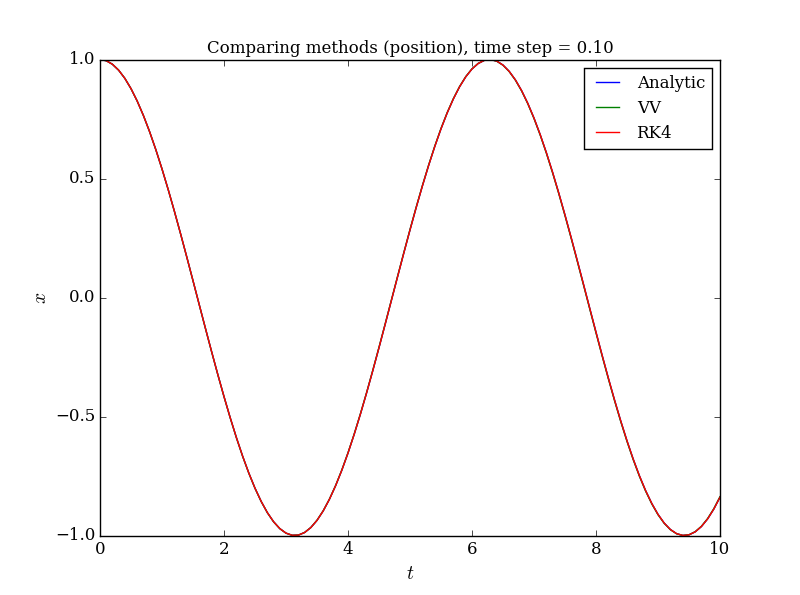
\includegraphics[width=90mm]{Images/comparison_x_01.png}
	& 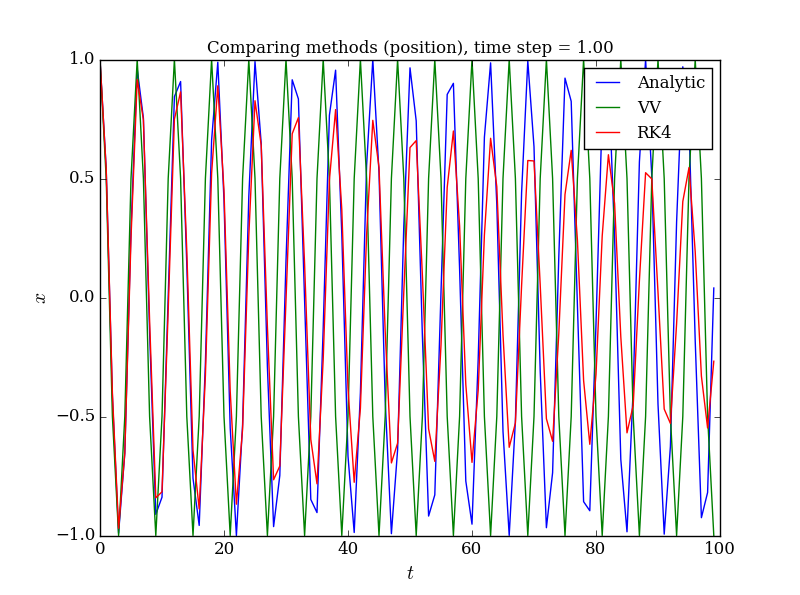
\includegraphics[width=90mm]{Images/comparison_x_1.png} \\
	(a) Position, $\Delta t = 0.10$, $t_{\mathrm{final}} = 10$				& (b) Position, $\Delta t = 1.00$, $t_{\mathrm{final}} = 100$  \\[6pt]
	
	  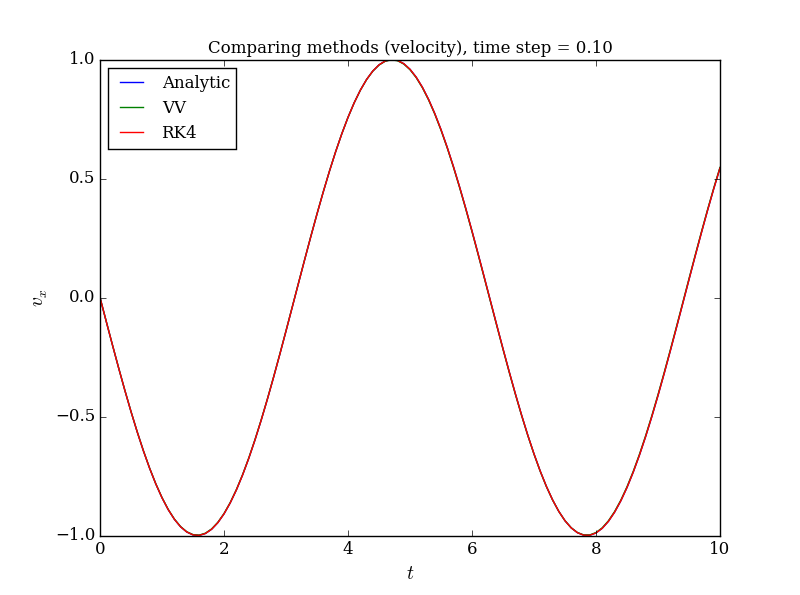
\includegraphics[width=90mm]{Images/comparison_v_01.png}
	& 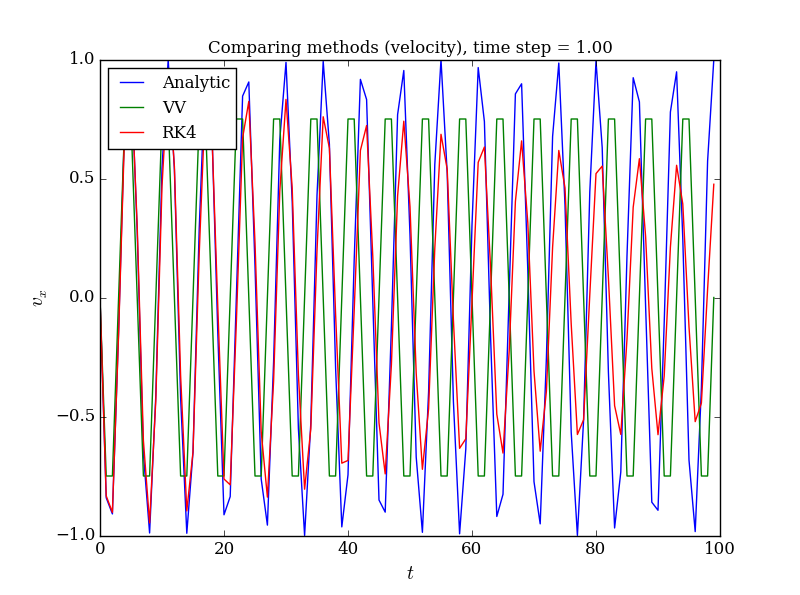
\includegraphics[width=90mm]{Images/comparison_v_1.png} \\
	(c) Velocity, $\Delta t = 0.10$, $t_{\mathrm{final}} = 10$				& (d) Velocity, $\Delta t = 1.00$, $t_{\mathrm{final}} = 100$  \\[6pt]
	
  	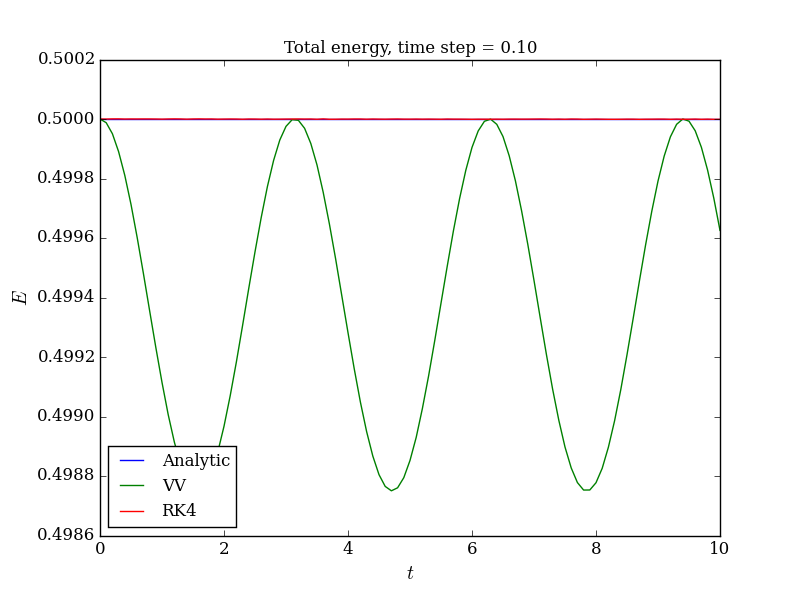
\includegraphics[width=90mm]{Images/comparison_E_01.png}
	& 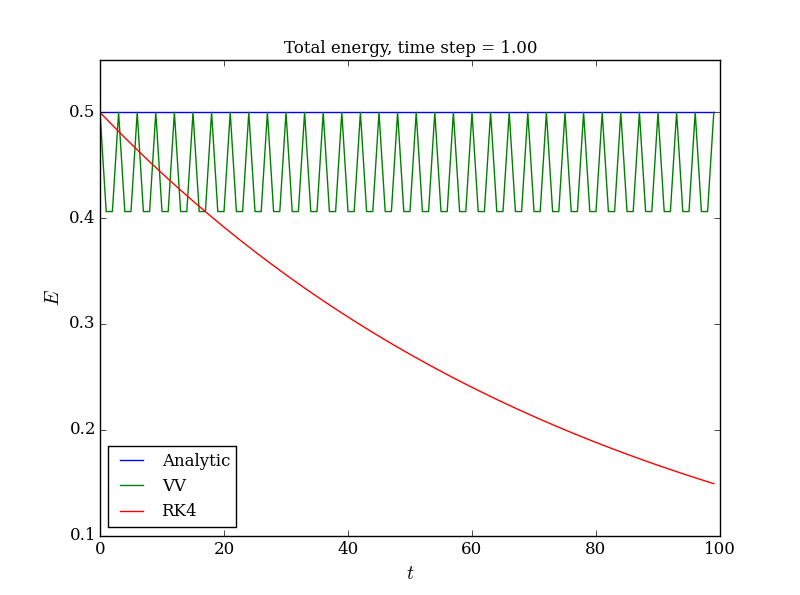
\includegraphics[width=90mm]{Images/comparison_E_1.png} \\
	(e) Energy, $\Delta t = 0.10$, $t_{\mathrm{final}} = 10$				& (f) Energy, $\Delta t = 1.00$, $t_{\mathrm{final}} = 100$  \\[6pt]
\end{tabular}
\caption{Comparison of our numerical algorithms in the analytical case of the box on a spring: Velocity-Verlet (green) and 4th-order Runge-Kutta (red), with the analytical solution (blue) are shown for two different time steps $\Delta t = 0.10$ and $\Delta t = 1.00$, and for two different durations $t_{\mathrm{final}} = 10$ and $t_{\mathrm{final}} = 100$.}\label{fig:analytical}
\end{center}
\end{figure*}


\noindent Now that we have verified our numerical methods, we can go on to solve the problem at hand.



\subsection{Stability of methods}

% Spring force
Let us first comment on the stability of the analytical case before moving on to the gravitational system. Studying the analytical case with spring force, the two methods described in Sec.~\ref{sec:methods} are good estimates for time step $\Delta t<1$. RK4 is slightly closer to the analytical solution. For $\Delta t \geqslant 1$, the oscillation in position and velocity is damped when using RK4. This is more visible for longer times. With the VV method, the position amplitude is 1, whereas the velocity amplitude is lowered to 0.75. Thus, for larger time steps, VV is the most stable method.

% 2-body problem
Now let us consider the Newtonian two-body problem in three dimensions. Here we have chosen a configuration close to that of the Sun-Earth system: One mass is heavy and has no velocity of its own (Sun-like object), while the other mass is much lighter with some velocity in the $x$-direction (Earth-like object). By trying out different relative distances $r$ between the Sun-like and the Earth-like object, as well as different velocities in the $x$-direction, we can get a system where our Earth-like object follows a nice orbit around the massive object in the center. As seen in Fig.~\ref{fig:2_body}a-d, the orbit -- or lack thereof -- very much depends on the time step, especially in the case where the radius is a bit too small to make the orbit stable, visible in Fig.~\ref{fig:2_body}b. In general it is clear from the figures that RK4 does a better job in all cases, except in Fig.~\ref{fig:2_body}c where the two methods give approximately identical results. 

\begin{figure*}
\begin{center}
\begin{tabular}{cc}
  	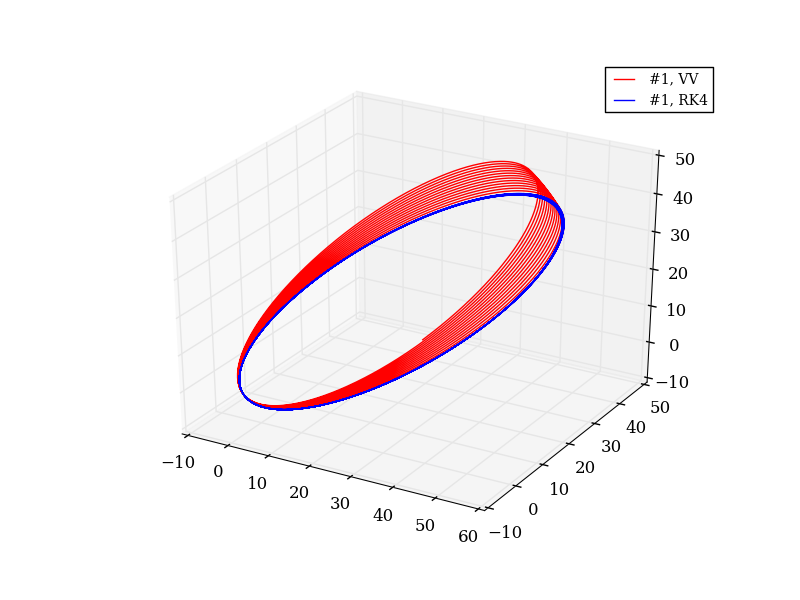
\includegraphics[width=90mm]{Images/comparison_orbit_01_dist40.png}
	& 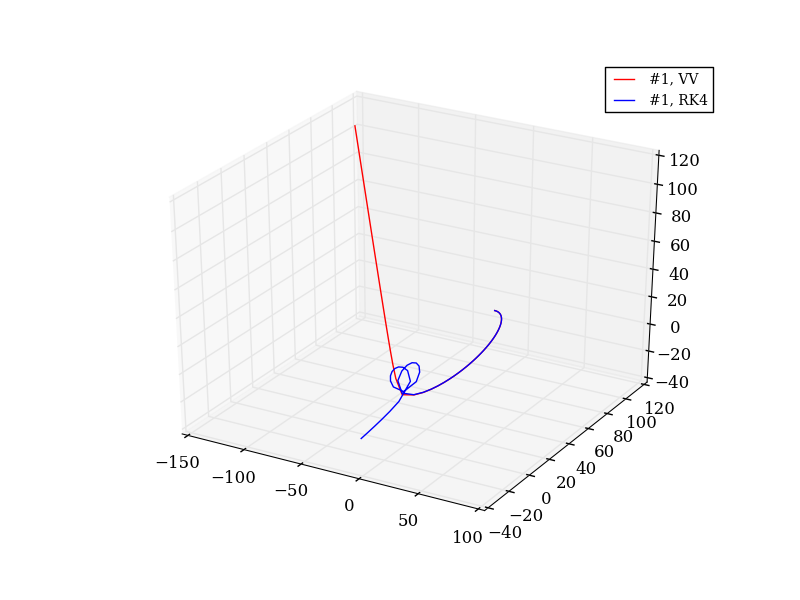
\includegraphics[width=90mm]{Images/comparison_orbit_1_dist40.png} \\
	(a) $\Delta t = 0.10$, $t_{\mathrm{final}} = 1\,000$, $r = 40$				& (b) $\Delta t = 1.00$, $t_{\mathrm{final}} = 1\,000$, $r = 40$  \\[6pt]
	
	 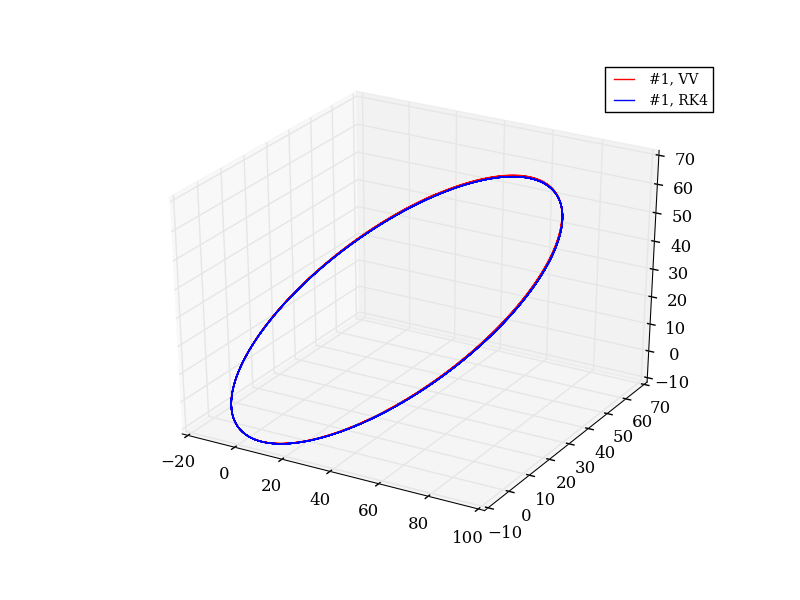
\includegraphics[width=90mm]{Images/comparison_orbit_01_dist60.png}
	& 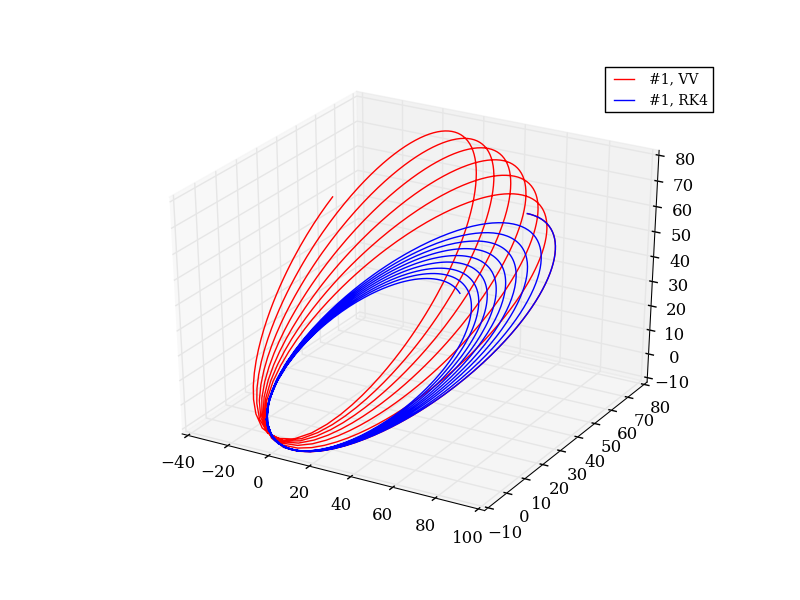
\includegraphics[width=90mm]{Images/comparison_orbit_1_dist60.png} \\
	(c) $\Delta t = 0.10$, $t_{\mathrm{final}} = 1\,000$, $r = 60$				& (d) $\Delta t = 1.00$, $t_{\mathrm{final}} = 1\,000$, $r = 60$  \\[6pt]
	
	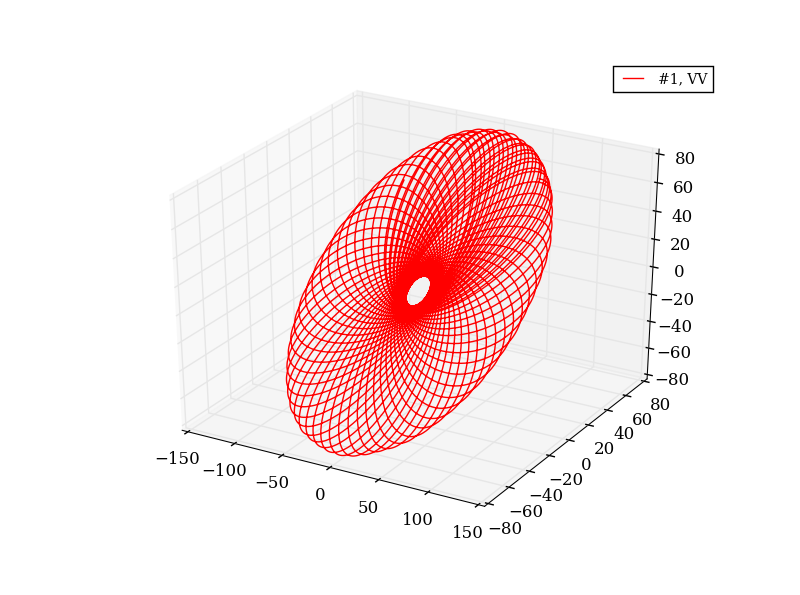
\includegraphics[width=90mm]{Images/VV_longtime.png}
	& 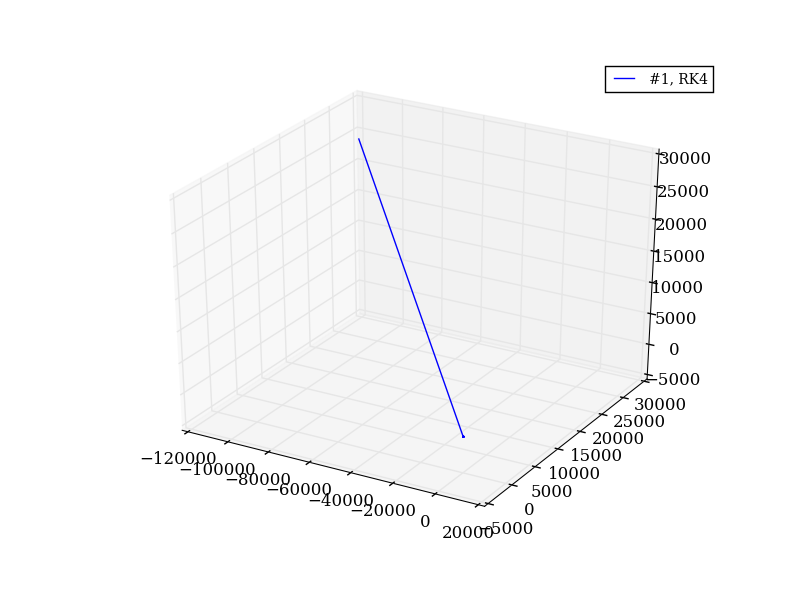
\includegraphics[width=90mm]{Images/RK_longtime.png} \\
	(e) $\Delta t = 1.00$, $t_{\mathrm{final}} = 10\,000$, $r = 60$				& (f) $\Delta t = 1.00$, $t_{\mathrm{final}} = 10\,000$, $r = 60$  \\[6pt]
\end{tabular}
\caption{Orbits for our two numerical algorithms in the 2-body case where one body is massive and sitting in the center of the orbit (not plotted): Velocity-Verlet (red) and 4th-order Runge-Kutta blue for two different time steps $\Delta t = 0.10$ and $\Delta t = 1.00$, as well as two different radii, $r = 40$ and $r = 60$ and two different final times $t_{\mathrm{final}} = 1\,000$ and $t_{\mathrm{final}} = 10\,000$.}\label{fig:2_body}
\end{center}
\end{figure*}
When choosing the final time to be $t = 10\,000$, however, VV proved is the most stable method, as seen in Fig.~\ref{fig:2_body}e-f, as the star that went through the RK4 method was ejected. 

What is also interesting is to compare the time used by the two different methods to see which one is the most efficient:

\begin{center}
\begin{tabular}{ l l l l }\hline
	$\Delta t$ 				& Integration points	 	& Time RK4 (s)		& Time VV (s)		\\ \hline
	1.0 					& $10 \, 000$ 			& 0.349			& 0.326		 \\
	0.1 					& $1 \, 000$			& 3.477 			& 4.300		 \\
	\hline
\end{tabular}
\end{center}
We see that the time usage is very similar for the two methods, with VV being slightly more efficient for a large time step, and RK4 being the most efficient for a small time step. 

Finally we want to see whether energy is conserved for our star. This is done calculating

\begin{equation}\label{eq:E_tot}
	E = \frac{1}{2}Mv^2 - \frac{GM^2}{r}
\end{equation}
where $M$ is the mass of the light, orbiting star with velocity $v$ and position $r$. The first term represents the kinetic energy and the second term represents the potential energy. The result for the two methods is shown in Fig.~\ref{fig:2_body_energy}. We see that COMMENT!

In conclusion, based on our study of the stability, time usage and energy conservation of the two methods, we can say that VV would be the better choice of method when simulating systems that require long times.


\begin{figure*}
\begin{center}
\begin{tabular}{cc}
  	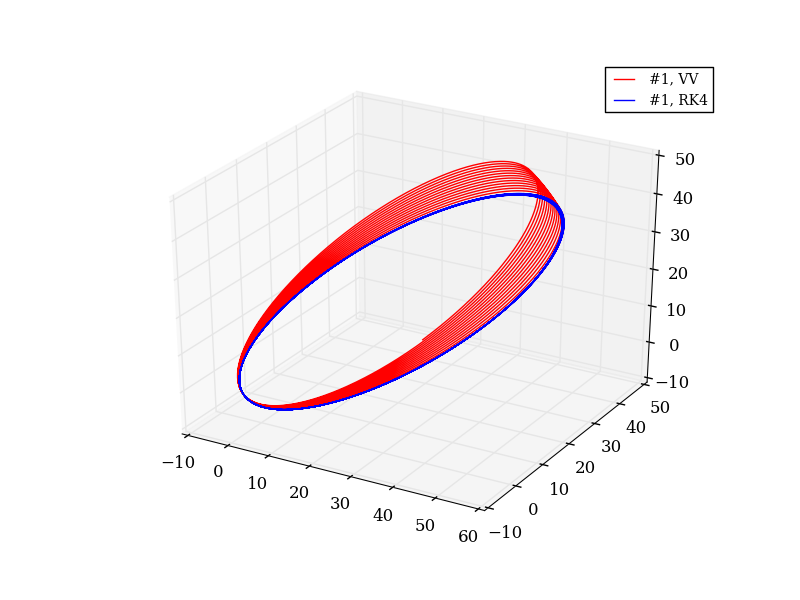
\includegraphics[width=90mm]{Images/comparison_orbit_01_dist40.png}
	& 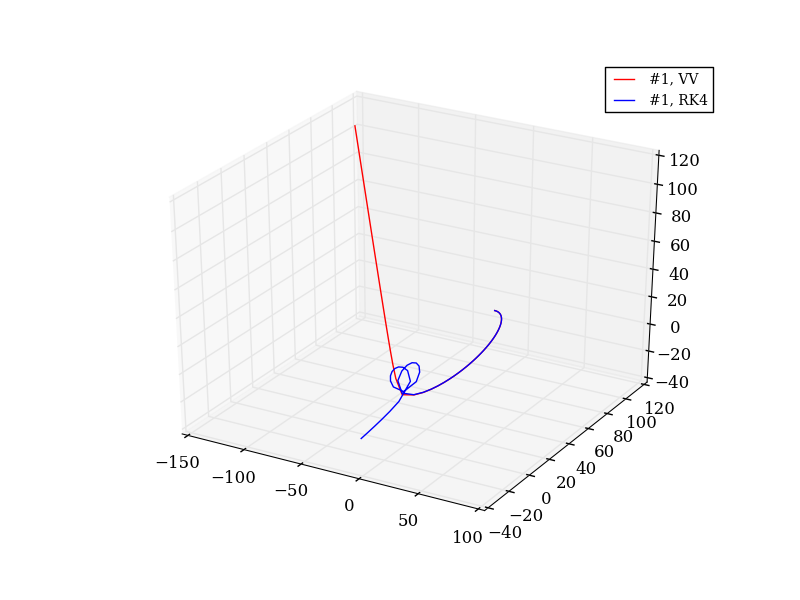
\includegraphics[width=90mm]{Images/comparison_orbit_1_dist40.png} \\
	(a) $\Delta t = 0.10$, $t_{\mathrm{final}} = 1\,000$, $r = 40$				& (b) $\Delta t = 1.00$, $t_{\mathrm{final}} = 1\,000$, $r = 40$  \\[6pt]
\end{tabular}
\caption{Energy conservation for our two numerical algorithms in the 2-body case where one body is massive and sitting in the center of the orbit (not plotted): Velocity-Verlet (red) and 4th-order Runge-Kutta blue for two different time steps $\Delta t = 0.10$ and $\Delta t = 1.00$, as well as two different radii, $r = 40$ and $r = 60$ and two different final times $t_{\mathrm{final}} = 1\,000$ and $t_{\mathrm{final}} = 10\,000$.}\label{fig:2_body_energy}
\end{center}
\end{figure*}



\subsection{Evolution of the $N$-body system}
We go on to study the $N$-body system. For a system with $N = 100$ objects and a radius $R_0$ = 20 ly, we want to know how large the time steps are required to be. We run the calculations for both methods in Sec.~\ref{sec:methods} for different time steps to see how a change in time step while change the results.

In the case where the number of objects $N \rightarrow \infty$ and the mean density $\rho_0$ is kept constant, the system would collapse into a singularity at a finite \textbf{collapse time} because it can be considered a continuous fluid. Then each imaginary shell for different radii from the center will be fully filled and feel the same gravitational force towards the center of the system, thus reaching the center at the same time. 

This will not be the case in our model where $N$ is finite. Then the gravitational field will be largely non-uniform, which means the objects will be pulled towards the center of the system and reach it at different times, and keep moving to the other side of the center, instead of all particles gathering in the center at the same time, creating a collapse. This we can see in Fig. XXX.

COMMENTS.


\subsubsection{The energy of the system}

We calculate the kinetic and potential energy of our system using Eq. (\ref{eq:E_tot}) to study whether the energy is conserved, and see if this is dependent on the number of objects $N$.

MORE!!!



\subsubsection{Introducing the smoothing function}

After running calculations for the gravitational force as expressed in Eq. (\ref{eq:force_comp}), we introduce a smoothing function to take care of any numerical instability that may arise when two stars come very close. We modify the gravitational force as

\begin{equation}\label{eq:force_mod}
	F_{G,\mathrm{mod}} = - \frac{G M_1 M_2}{r^2 + \epsilon^2},
\end{equation}
where $\epsilon$ is a small real constant. We will try out different values for $\epsilon$ to see which value gives the best energy conservation.

MORE!!!




\subsubsection{Testing the virial theorem}

The \textbf{virial theorem} says that for a bound gravitational system in equilibrium we have

\begin{equation}\label{eq:vir}
	2 \langle K \rangle = - \langle V \rangle,
\end{equation}
where $\langle K \rangle$ is the time-averaged kinetic energy of the system and $\langle V \rangle$ is the time-averaged potential energy of the system. The virial theorem deploys the ergodic hypothesis, which states that we can take an ensemble average instead of a time average. By calculating the kinetic and potential energy of the stars in our system that are bound (not ejected), we can check if our results are consistent with Eq. (\ref{eq:vir}).

MORE!!



\subsubsection{Radial profile}

Finally we wish to study the \textbf{radial density} of the particles in the equilibrium state. This can be calculated from our computations and be fitted with the simple expression

\begin{equation}\label{eq:simple_fit}
	n(r) = \frac{n_0}{1 + (\frac{r}{r_0})^4}
\end{equation}
where $n_0$ and $r_0$ are scaling constants. The result can also be compared with the well-known Navarro-Frenk-White profile

\begin{equation}\label{eq:NFW}
	\rho(r) = \frac{\rho_0}{  \frac{r}{r_0} (1 + \frac{r}{r_0})^2  },
\end{equation}
where $\rho_0$ and $r_0$ are scaling constants. 

MORE!!!






\section{Conclusions}

...




\section{List of codes}

The codes developed and used in this project are: 


\subsection{Running calculations (C++)}

\begin{itemize}
	\item \verb@main.cpp@ -- main program where the calculations are run, calling on the classes listed below. 
	\item \verb@star.cpp@ -- class collecting various properties of the stars.
	\item \verb@galaxy.cpp@ -- class containing all the stars in the galaxy as well as the numerical methods described in Sec.~\ref{sec:methods}.
\end{itemize}


\subsection{Plotting (Python)}

\begin{itemize}
	\item \verb@plotting_analytical.py@ -- program to graphically compare the one-dimensional 2-body problem with an analytical solution, described in Sec.~\ref{sec:analytical_test}.
	\item \verb@plot_method.py@ -- program to graphically compare the two numerical methods described in Sec.~\ref{sec:RK4} and Sec.~\ref{sec:VV} for the 2-body problem.
	\item \verb@plot_method_Nbody.py@ -- program to graphically compare the two numerical methods for the $N$-body problem.
	\item \verb@plotting_scatter.py@ -- plotting program to visualize the 3D distribution of particles in the $N$-body system as a scatter plot. 
	\item \verb@plotting_radialprofile.py@ -- plotting program that calculates the radial profile of the system, fitted with the profiles in Eq. (\ref{eq:simple_fit}) and Eq. (\ref{eq:NFW}).
\end{itemize}




\end{multicols}

\end{document}
